\section{Implementazione}\label{sec:implementazione}

\subsection{Linguaggi e strumenti}
\subsubsection{HTML}
La struttura e il contenuto del sito sono stati realizzati attraverso il linguaggio \textit{HTML5}. Questa scelta è stata fatta per due principali ragioni:
\begin{enumerate}
	\item Trattandosi di un sito di vendita online, è importante che tutte le pagine siano le più coerenti possibile in modo da poter competere nel mercato con un sito fatto bene ed aggiornato. Inoltre, avere pagine scritte con linguaggi recenti aiuta moltissimo nella leggibilità del codice ed è più facile modificarlo.
	\item Un altro motivo per il quale si è scelto \textit{HTML5} è relativa all'utenza finale. Essendo principalmente le generazioni più giovani quelle ad affidarsi al mondo online per fare acquisti, i dispositivi e i motori di ricerca utilizzati saranno tendenzialmente più recenti.
	\end{enumerate}
	Si è comunque mantenuta la compatibilità con \textit{XHTML}, permettendo al sito di essere pienamente funzionante anche sui \textit{browser} più vecchi ed obsoleti. Durante tutto il processo di progettazione e creazione delle pagine si sono utilizzate le linee guida del corso di Tecnologie Web e quelle del \textit{W3C}. Il codice è stato validato utilizzando il tool di validazione del \href{https://validator.w3.org/}{W3C}.
Alcune delle regole più importanti sono:
\begin{itemize}
	\item \textbf{Separazione della struttura, presentazione e contenuto}: Non ci devono essere file \textit{script} oppure fogli di stile nel codice \textit{HTML}. Questi devono essere scritti in file esterni e poi importati nell’\textit{header} delle pagine \textit{HTML}.
	\item \textbf{Tag}: Tutti i \textit{tag} devono essere chiusi e si devono utilizzare i \textit{tag} che migliorano l'accessibilità del sito.
	\item \textbf{Metatag}: L’inserimento dei \textit{metatag} nella sezione head è molto importante in quanto migliora l’accessibilità del sito verso i browser. Allo stesso tempo, l’utilizzo corretto delle \textit{keyword} aiuta in un ranking migliore nella ricerca.
	\item \textbf{Tabelle}: Le tabelle devono essere sempre evitate, oppure rese accessibili se il loro utilizzo è essenziale.
\end{itemize}

\subsection{PHP}
Il lato server del sito viene gestito da file \textit{PHP} che stabiliscono il comportamento generale delle pagine, interagiscono con il \textit{database} e creano le sessioni di utilizzo per gli utenti loggati. Per agevolare l’interazione con il \textit{database}, sono state create delle classi di supporto che vanno a modellare i record delle principali tabelle del \textit{database}.

\textbf{File dp.php}: Questo file contiene le classi e le funzioni che fanno da intermediari tra gli script PHP e le chiamate al database. Si occupa principalmente di:
	\begin{itemize}
		\item Gestire la connessione con il \textit{database}
		\item Fornire funzioni per il recupero dei dati dal \textit{database}
		\item Fornire funzioni per l’inserimento, la modifica e la cancellazione di dati nelle tabelle
	\end{itemize}
	
\textbf{File response\_manager.php}: Contiene la classe \textit{response\_manager} che fornisce metodi necessari per la gestione delle risposte e il controllo degli errori.

\textbf{"nomepagina".php:} (esempio: \textit{bestseller.php, generi.php}) sono i file che costruiscono le pagine del sito. Utilizzano le rispettive pagine html (es: \textit{bestseller\_php.html}) che contengono l’effettivo \textit{html}.

Quasi tutte hanno una procedura di esecuzione standard:
\begin{enumerate}
	\item Verificano i permessi dell’utente
	\item Verificano la disponibilità di connessione al \textit{database}
	\item Richiedono le informazioni necessarie per la operazione da effettuare al \textit{database}
	\item Eseguono l'operazione della modifica del database richiesta dall’utente che può essere un inserimento, modifica o cancellazione di dati
\end{enumerate}

In alcune pagine vengono effettuate delle validazioni sintattiche e di dominio prima di eseguire l’inserimento o la modifica dei dati. La validazione sintattica cerca di individuare la presenza di errori che potrebbero impattare sull'esito della \textit{query}, mentre quelle di dominio mirano ad evitare l’inserimento di informazioni non coerenti nel database (esempio: aggiungere più articoli al carrello della quantità disponibile per ciascuno).

Un altro aspetto importante sul quale ci siamo focalizzati è la sicurezza dell'area privata. Sono stati aggiunti controlli che non permettono a tipi di utenti diversi di accedere ai contenuti di un altro tipo. Quindi un utente loggato non può accedere ai contenuti dell’admin e l’admin non può accedere ai contenuti di un utente registrato.

Attraverso questo controllo si riesce inoltre ad impedire l’accesso all’area riservata senza aver effettuato il \textit{login}.

\subsection{CSS}
Il \textit{layout} del sito è stato modellato utilizzando la versione 3 del linguaggio di formattazione \textit{CSS}. Come descritto anche nel caso del \textit{HTML5}, essendo gli utenti principali del sito persone relativamente giovani, possiamo assumere l’utilizzo dei motori di ricerca moderni nella maggioranza dei casi.

Sono stati prodotti 4 fogli di stile differenti, ciascuno per un opportuno dispositivo: \textit{style.css, medium.css , mini.css e print.css} (per la stampa) che contengono all'interno tutte le clausole relative alla formattazione dei documenti e varie regole disponibili con \textit{CSS3} come: \textit{flexbox}, variabili, selettori ecc.

Come strategia di progettazione abbiamo usato \textit{Responsive Web design} basata sul concetto di \textit{media query} che ottimizzano la visualizzazione in base a dispositivi specifici e dimensioni di \textit{viewport}. Grazie all’utilizzo di misure sempre \textit{relative} o in \textit{percentuale} è stato implementato un design fluido e scalabile, che permette una corretta visualizzazione delle pagine su tutti i formati di schermo, senza intaccare in alcun modo la navigazione tramite \textit{screen reader}. Così facendo si migliora anche l’accessibilità del sito.

\subsection{SQL}
Il linguaggio SQL è stato utilizzato per la codifica del \textit{database} il quale è composto dalle seguenti tabelle:
\begin{itemize}
	\item \textbf{libro:} la tabella contenente tutti i libri che sono stati aggiunti dal admin e che sono ancora in vendita. I campi sono: \textit{isbn, titolo, editore, pagine, prezzo, quantità, data\_pubblicazione, percorso, trama} che descrive brevemente di cosa parla il libro
	\item \textbf{editore:} contiene i \textit{nomi} delle diverse case editrici e l’\textit{id}. Ci possono essere più di un libro pubblicati dalla stessa casa
	\item \textbf{autore:} contiene l’\textit{id, nome e cognome} dell'autore del libro. Un libro può avere più di un autore e un autore può aver pubblicato più di un libro
	\item \textbf{pubblicazione:} è la relazione tra un libro e il suo/suoi autori. Contiene i campi \textit{libro\_isbn} e \textit{autore\_id}.
	\item \textbf{categoria:} contiene la lista delle categorie (generi) presenti. Campo \textit{id\_categoria} e \textit{nome}
	\item \textbf{appartenenza:} è la relazione tra un libro e la categoria in cui fa parte. Ci sono libri che fanno parte in più di una categoria. Campi \textit{libro\_isbn} e \textit{codice\_categoria}
	\item \textbf{offerte:} contiene la lista dei libri che sono in offerta. Campi \textit{libro\_isbn, data\_inizio, data\_fine}, e \textit{sconto} che indica la percentuale dello sconto applicato
	\item \textbf{utente:} contiene i campi in cui si salvano i dati degli utenti registrati e dell'amministratore; \textit{codice\_identificativo, nome, cognome, data\_nascita, username, email, password, telefono}
	\item \textbf{ordine:} contiene \textit{codice\_univoco, cliente\_codice} che è il \textit{codice\_identificativo} dell’utente che ha effettuato l’\textit{ordine, data, data\_partenza, data\_consegna, indirizzo, totale}
	\item \textbf{composizione:} è la relazione tra la tabella ordini e libro. Contiene i campi \textit{elemento, codice\_ordine, quantità}
	\item \textbf{wishlist:} dove vengono memorizzati gli elementi aggiunti alla wishlist, contiene i campi \textit{cliente\_codice e libro\_isbn}
	\item \textbf{indirizzo:} tabella con campi \textit{codice, via, città, cap, num\_civico, utente} a cui corrisponde l’indirizzo
	\item \textbf{recensioni:} tabella che contiene le recensioni dell'utente. Campi \textit{id\_utente, libro\_isbn, data\_inserimento, valutazione e commento}
\end{itemize}

\begin{figure}[h]
	\centering
	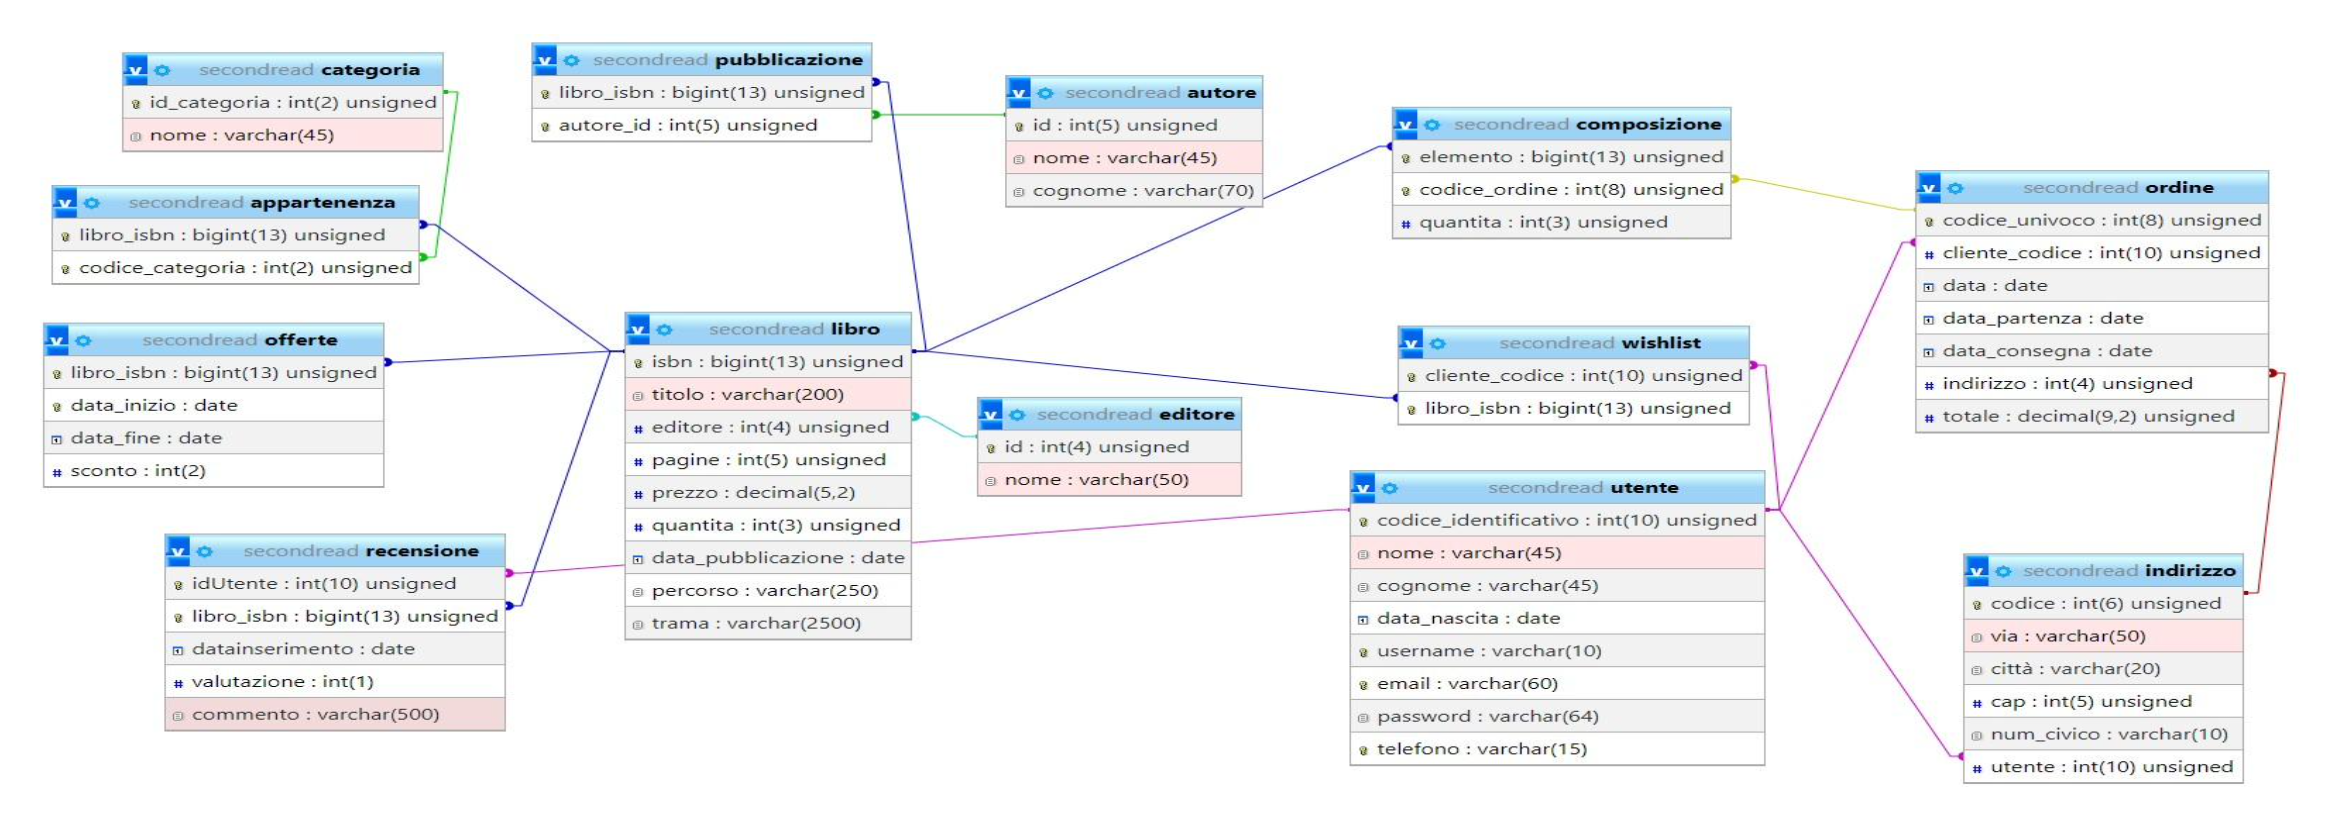
\includegraphics[scale=0.4]{images/er_db}
	\caption{Schema ER del \textit{database}}
\end{figure}

\subsection{Javascript}
Per il comportamento di determinate pagine del sito, sono stati utilizzati file JavaScript che contengono varie funzioni necessarie per il controllo dell’\textit{input nei form}. Attraverso l’utilizzo di espressioni regolari sono stati effettuati i necessari controlli di validità su tutti gli \textit{input}.

Il controllo è stato effettuato sia nella parte pubblica che nella parte privata ( utente e amministratore). È stato indispensabile l’utilizzo di javascript anche nella configurazione dei bottoni. Ad esempio, è stato creato un apposito script per i bottoni dei \textit{filtri} della ricerca (\textit{Reset, PrezzoMin} e \textit{PrezzoMax}), per il bottone Torna Su e per tutti i bottoni delle altre pagine interattive (\textit{Registrati, Accedi, Acquista, Aggiungi al carrello, Aggiungi alla wishlist, Applica sconto...})

Abbiamo creato uno script anche per la configurazione della \textit{navbar} laterale (\textit{burgerMenu.js}), dove sono state sviluppate le funzioni utili per la sua apertura e la chiusura.

Il pulsante del \textit{burger-menu} e poi anche \textit{X} che serve a chiuderla, sono situati in alto a destra delle pagine.

\subsection{XAMPP}
Il corretto funzionamento della parte dinamica, particolarmente PHP e SQL, è stato verificato tramite \textit{XAMPP}. Questo ha reso possibile testare il sito con dispositivi mobile, aprendo la porta 80 dalla propria macchina e rendendo il tutto accessibile nella rete locale.

Così facendo è stato possibile testare meglio il \textit{layout} e i bottoni in modo da evitare il \textit{fat finger}.

\subsection{Chrome Inspect}
La modalità Ispeziona di \textit{Chrome} è stata usata maggiormente per testare \textit{CSS} e \textit{HTML} rendendo il processo di \textit{debugging} più facile. Inoltre, grazie alla possibilità di cambiare gli attributi del CSS senza modificarli nei file originali è stato più semplice decidere quale approccio seguire in alcuni casi di indecisione.

